\section{Evaluation}
\label{sec:dda:eval}


This section evaluates the prediction accuracy of \name (Section~\ref{subsec:accuracy-eval}) and how much \name improves video bitrate (Section~\ref{subsec:bitrate-eval}). Overall, our findings show the following: 
\begin{packedenumerate}
\item \name can predict more accurately than other predictors.
\item With higher accuracy, \name can select better bitrate.
\end{packedenumerate}

\subsection{Prediction Accuracy}
\label{subsec:accuracy-eval}


\myparatight{Methodology} As points of comparison, we use implementations of Decision Tree (DT) and Naive Bayes (NB) with default configurations in \texttt{weka}, a popular ML tool~\cite{weka}. For a fair comparison, all algorithms use the same set of features. We also compare them with last-mile predictor (LM)\footnote{LM is not applicable to the VoD dataset as it has no feature related to last-mile connection.} and last-sample predictor (LS), introduced in Section~\ref{sec:dda:back}. We update the model of other algorithms in a same way as \name: for each session under prediction, we use all available history data before it as the train data. Each session's timestamp is grouped into 10-minute intervals and used as discrete time feature. By default, we use absolute normalized error (Section~\ref{sec:dda:design}) as the metric of prediction error, and the results are based on the FCC dataset, unless specified otherwise.

\mypara{Distribution of prediction error} Figure~\ref{fig:prediction-error} shows the distribution of prediction error of \name and other algorithms.
\name outperforms all algorithms, especially on the tail of prediction error. For the FCC dataset (Figure~\ref{fig:prediction-error-fcc}), 80\%ile prediction error of \name is 50\% to 80\% lower than that of other algorithms, and \name has less than 20\% sessions with more than 10\% prediction error, while all other algorithms have at least 30\% session with more than 10\% error. While the VoD dataset in general has higher prediction error than the FCC dataset (due to the lack of some features such as last-connection and longitudinal information), \name still outperforms other algorithms, showing that \name is robust to the available features.

\begin{figure}[h!]
\centering
%\hspace{-0.6cm}
\subfloat[FCC]
{
        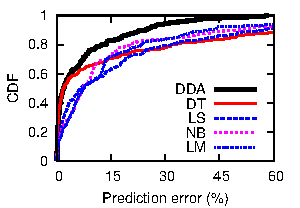
\includegraphics[width=0.46\textwidth]{figures/dda-temp-CDF.pdf}
        \label{fig:prediction-error-fcc}
}
%\hspace{-0.6cm}
\subfloat[VoD China]
{
        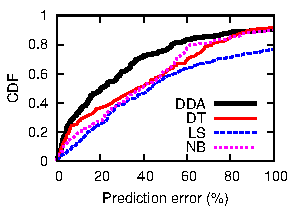
\includegraphics[width=0.46\textwidth]{figures/dda-temp-CDF-pptv.pdf}
        \label{fig:prediction-error-pptv}
}
%\hspace{-0.6cm}
\caption{CDF of prediction error.}
\label{fig:prediction-error}
\end{figure}



\begin{figure*}[t!]
\centering
%\hspace{-0.6cm}
\subfloat[Prediction error vs. ISP]
{
        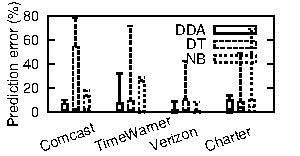
\includegraphics[width=0.44\textwidth]{figures/dda-temp-partition-ISP.pdf}
        \label{fig:insight-isp}
}
%\hspace{-0.6cm}
\subfloat[Prediction error vs. time of day (UTC)]
{
        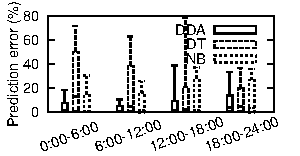
\includegraphics[width=0.44\textwidth]{figures/dda-temp-partition-time.pdf}
        \label{fig:insight-timeofday}
}\\
%\hspace{-0.6cm}
\subfloat[Prediction error vs. random drop rate]
{
        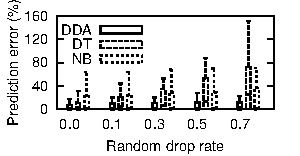
\includegraphics[width=0.44\textwidth]{figures/dda-temp-sensitivity.pdf}
        \label{fig:sensitivity}
}
%\hspace{-0.6cm}
\caption{Dissecting \name prediction error. The boxes show the 10-20-50-80-90 percentile.}
\label{fig:insight}
\end{figure*}

\mypara{Dissecting prediction accuracy of \name} To evaluate the prediction accuracy in more details, we first partition the prediction error by four most popular ISPs (\ref{fig:insight-isp}) and by different time of day (\ref{fig:insight-timeofday}). Although the ranking of algorithms varies across different partitions, \name consistently outperforms other two algorithms (DT, NB), especially in the tail of 90\%ile. Finally, Figure~\ref{fig:sensitivity} evaluates \name's sensitivity to measurement frequency by comparing the distribution of prediction error of three algorithms under different random drop rates (Section~\ref{subsec:dataset}). It shows that \name is more robust to measurement frequency than the other algorithms.
%When random drop rate is zero, the measurement frequency between each client and target is once every hour, and when random drop rate is 0.5, the measurement frequency between each client and target is in average once every 2 hours. 

%the FCC dataset has one measurement between a client and target every hour, and this allows us to evaluate the prediction accuracy under different measurement frequency. To do this, we randomly drop part of the measurement in the FCC dataset, and Figure~\ref{fig:sensitivity} shows the average prediction error and their distribution of three prediction algorithms under different random drop rate. When random drop rate is zero, the measurement frequency between each client and target is once every hour, and when random drop rate is 0.99, the measurement frequency between each client and target is in average once every 100 hours. First, Figure~\ref{fig:sensitivity-mean} shows that the average prediction error of \name is more robust to measurement frequency than the other algorithms (NN and NB). Second, Figure~\ref{fig:sensitivity-distribution} shows that the tails (10,20,80,90 percentile) of prediction error \name is much more stable than the other algorithms against measurement frequency.


\subsection{Improvement of Bitrate Selection}
\label{subsec:bitrate-eval}

%This section shows the bitrate improvement resulted from accuracy throughput prediction of \name. 

\mypara{Methodology} To evaluate bitrate selected based on some prediction algorithm, we consider a simple bitrate selection algorithm (while a more complex algorithm is possible, it is not the focus of this paper): given a session of which the prediction algorithm predicts the throughput by $w$, the bitrate selection algorithm simply picks highest bitrate from \{0.016, 0.4, 1.0, 2.5, 5.0, 8.0, 16.0, 35.0\}Mbps~\cite{youtube-bitrates} and below $\alpha w$, where $\alpha$ represents the safety margin (e.g.,  higher $\alpha$ means higher bitrate at the risk of exceeding the throughput). We use two metrics to evaluate the performance: (1) AvgBitrate -- average value of picked bitrate, and (2) GoodRatio -- percentage of sessions with no re-buffering (i.e., picked bitrate is lower than the throughput). Therefore, one bitrate selection algorithm is better than another if it has both higher AvgBitrate and higher GoodRatio.
As points of reference, ``Global'' bitrate selection algorithm picks the same bitrate for any session, which represents how today's players select starting bitrate. As a optimal reference point, ``Ideal'' bitrate selection algorithm picks the bitrate identical to the throughput for any session (Section~\ref{subsec:dataset}).

\mypara{Overall improvement} Table~\ref{tab:bitrate-overall} compares \name-based bitrate selection and the ``Global''. In both algorithms, we use $\alpha=0.8$ for the FCC dataset, and $\alpha=0.6$ for the VoD dataset. In both datasets, \name leads to higher AvgBitrate and GoodRatio, and \name is much closer to ``Ideal'' than ``Global''. Note that the VoD dataset still has a substantial room of improvement due to the relatively low prediction accuracy (Figure~\ref{fig:prediction-error-pptv}).

\begin{table}[t]
%\begin{footnotesize}
\begin{tabular}{l|l|l|l|l}
       & \multicolumn{2}{c}{{\bf FCC}} & \multicolumn{2}{c}{{\bf VoD China}} \\ 
       & {\bf AvgBitrate} & {\bf GoodRatio} & {\bf AvgBitrate} & {\bf GoodRatio} \\\hline\hline
Global &    2.5Mbps       &  88.2\%         & 2.5Mbps          &  77.5\%           \\
\name  &    13.3Mbps      &  99.5\%         & 2.7Mbps          &  88.2\%           \\
Ideal  &    27.2Mbps      &  100\%          & 3.5Mbps          &  100\%              
\end{tabular}
%\end{footnotesize}
\caption{Comparing \name and ``Global'' in AvgBitrate and GoodRatio.}
\label{tab:bitrate-overall}
\end{table}

\myparatight{Bitrate selection vs. prediction accuracy} Next, we examine the intuition that higher prediction accuracy leads to higher performance of bitrate selection. Table~\ref{tab:bitrate-accuracy} shows the bitrate selection performance as a function of median prediction error. We consider four prediction algorithms (\name, DT, LS, NB). For a fair comparison, the bitrate selection algorithm always uses $\alpha=0.8$. As prediction error increases, the performance of bitrate selection degrades in terms of both lower AvgBitrate and lower GoodRatio.


%\begin{figure}[h!]
%\centering
%\hspace{-0.6cm}
%\subfigure[Accuracy vs. AvgBitrate]
%{
%        \includegraphics[width=0.2\textwidth]{figures/bitrate-accuracy-bitrate.eps}
%        \label{fig:bitrate-accuracy-bitrate}
%}
%%\hspace{-0.6cm}
%\subfigure[Accuracy vs. GoodRatio]
%{
%        \includegraphics[width=0.2\textwidth]{figures/bitrate-accuracy-good.eps}
%        \label{fig:bitrate-accuracy-good}
%}
%\hspace{-0.6cm}
%\tightcaption{Higher accuracy means better bitrate selection.}
%\label{fig:bitrate-accuracy}
%\end{figure}

\begin{table}[t]
%\begin{footnotesize}
\begin{tabular}{p{0.8cm}|p{3.2cm}|p{2.5cm}|p{2.5cm}}
    & {\bf Mean/median prediction error} & {\bf AvgBitrate} & {\bf GoodRatio} \\ \hline\hline
\name & 9.0\%/2.3\%    & 13.3Mbps              & 99.5\%           \\
DT  & 23.1\%/3.4\%    & 13.0Mbps              & 91.0\%           \\
LS  & 28.7\%/9.8\%    & 12.3Mbps              & 90.6\%           \\
NB  & 91.4\%/17.1\%    & 12.2Mbps              & 71.8\%          
\end{tabular}
%\end{footnotesize}
\caption{Higher accuracy means better bitrate selection.}
\label{tab:bitrate-accuracy}
\end{table}

\mypara{Understanding bitrate improvement} There is a natural tradeoff between AvgBitrate and GoodRatio (e.g., higher $\alpha$ means higher AvgBitrate at the cost of lower GoodRatio). Figure~\ref{fig:bitrate-tradeoff} shows such tradeoff of various bitrate selection algorithms by adjusting the value $\alpha$. It is shown that \name-based bitrate selection strikes a better tradeoff of higher AvgBitrate and higher GoodRatio (i.e., more towards the top-right corner of the figure). 

Finally, we would like to test the robustness of \name-based bitrate selection in different regions. Figure~\ref{fig:bitrate-partition-isp} compares the AvgBitrate of \name with ``Global'' and ``Ideal'' in four popular ISPs. \name uses the maximum $\alpha$ on the tradeoff curve in Figure~\ref{fig:bitrate-tradeoff} that ensures at least 95\% GoodRatio, while ``Global'' only has GoodRatio of 88.2\%. 
Across all ISPs, \name consistently outperforms ``Global'' and achieve at least 60\% of the ``Ideal''.
%Comcast and Verizon have a large room of improvement (i.e., large gap between ``Global'' and ``Ideal''), and \name-based bitrate selection achieves close-to-ideal performance, resulting a higher improvement on these two ISPs. In contrast, there is substantial gap between \name and ``Ideal'' on Time Warner Cable and Charter, due to relatively higher prediction error (see Figure~\ref{fig:insight-isp}).


\begin{figure}[t!]
\centering
%\hspace{-0.6cm}
\subfloat[AvgBitrate-GoodRatio tradeoff]
{
        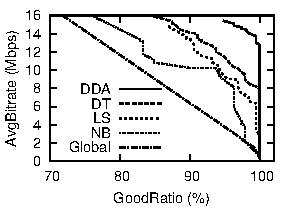
\includegraphics[width=0.44\textwidth]{figures/dda-bitrate-improvement-1.pdf}
        \label{fig:bitrate-tradeoff}
}
%\hspace{-0.6cm}
\subfloat[Performance by ISP]
{
        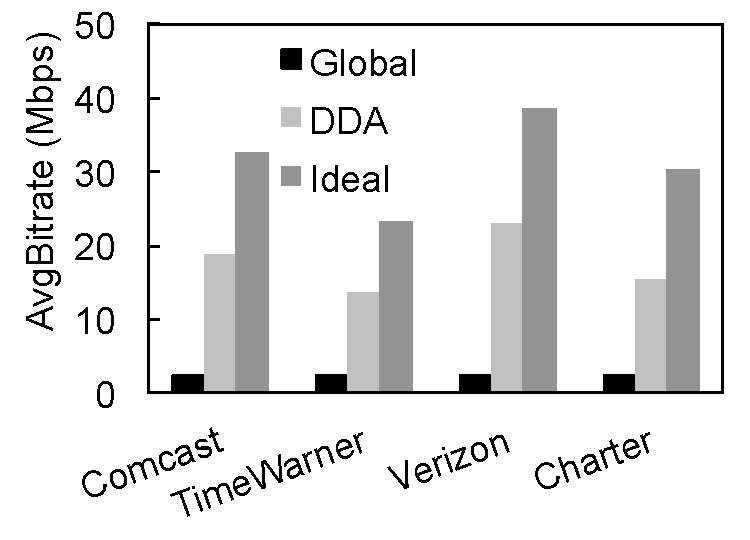
\includegraphics[width=0.44\textwidth]{figures/dda-bitrate-by-isp.pdf}
        \label{fig:bitrate-partition-isp}
}
%\hspace{-0.6cm}
\caption{In-depth analysis of bitrate selection}
\label{fig:bitrate-indepth}
\end{figure}

